% Milestone timeline for the historical development section.
% \input by chapters/02-literature-review.tex.
%
% LINEAR TIME AXIS: x = (year - 1932) * 0.155 cm, so 1932-2018 spans 13.3 cm.
% Ticks sit at the true year. There is deliberately no decade scale -- the
% spacing of the ticks themselves carries the elapsed time, and evenly spaced
% notches behind an unevenly spaced set of milestones read as a second, false
% rhythm. Every milestone prints its own year.
%
% Two tracks, because the section's claim is that PET inherited tomography
% rather than invented it:
%   tlpositron (blue)  -- the positron line proper
%   tlsingle (grey)    -- single-photon and transmission imaging (Anger, Kuhl,
%                         Hounsfield), the borrowed lineage
% TRACK MEMBERSHIP IS CARRIED BY COLOUR, NOT BY SIDE OF THE AXIS. Above is
% mostly positron and below mostly the borrowed lineage, but 1951 and 1989 are
% positron-line entries sitting below purely for room, as is 2013, and they
% stay blue. Do not "tidy" them to grey.
%
% LAYOUT -- a linear axis clusters 1951/1953 0.31 cm apart and 1973/1975/1976
% inside half a centimetre, so a label cannot sit above its own tick. Each
% entry therefore carries its own label position:
%
%     year / row / label x / text
%
% and a leader line slants from the tick to the label. Rows step outward from
% the axis in 1.50 cm increments. A 13.3 cm axis holds about five labels per
% row, so fourteen milestones need four rows in total. They are split two
% above and two below, which is what keeps the figure short -- an earlier
% version ran three rows above and two below and was 1.5 cm taller for it.
%
% TWO CLEARANCES, BOTH VERIFIED BY MEASUREMENT, NOT BY EYE. TeX warns about
% the page overrun but is completely silent about labels sitting on top of one
% another, and the first two attempts at this figure shipped with 1951/1953
% and 1958/1963 overlapping. Use the measurement hook at the foot of the file.
%
%   Horizontal -- labels are 2.3 cm wide (68.8 pt measured), so same-row
%   neighbours need their label x at least 2.6 cm apart. Current label x:
%     above row 1: 0, 3.2, 6.9, 9.5, 12.1
%     above row 2: 5.4, 8.19, 13.4    (set by leader routing, see below)
%     below row 1: 3.9, 6.6, 9.3, 12.2
%     below row 2: 2.3, 5.26          (set by leader routing, see below)
%   Tightest pairs are 1976/1986 and 1986/2006, both at 5.1 pt.
%
%   Vertical -- the row gap must exceed the TALLEST label, not the typical
%   one. Labels run to four lines when a long word will not fit the 2.3 cm
%   width (1953 is the worst at 47 pt), which is what broke an earlier
%   1.00 cm gap. At 1.50 cm the tightest pair is 2006 against row 2, with
%   3.5 pt of air.
%
%   Leaders crossing labels is a THIRD failure mode, not covered by either
%   check above. It is handled by the elbow routing described below, which is
%   what fixes the label x for every row-2 entry.
%
% Total extent -1.19 to 14.5 cm = 15.7 cm, inside the 16 cm text block.

\definecolor{tlpositron}{HTML}{2A6F97}
\definecolor{tlsingle}{HTML}{8B9BA4}
\definecolor{tltext}{HTML}{3D4A52}

% LEADERS ARE ELBOWS, NOT STRAIGHT LINES, AND THE ROUTE IS LOAD-BEARING.
%
% A straight leader from a tick out to row 2 cuts diagonally through the row-1
% band, and since a label (2.3 cm) is far wider than the tick spacing in the
% crowded stretches, it lands inside whichever row-1 label is nearest. That is
% what put visible breaks in five of the leaders: the white label fill was
% interrupting them.
%
% Instead each leader runs: up from the tick to y = 0.40, horizontally to its
% label's x, then straight up to the label. Both segments are in clear space:
%   - the horizontal run at 0.40 is below every label (labels start at 0.55)
%   - the vertical run is placed in a GAP between row-1 labels
% so no leader touches a label at all and none is interrupted.
%
% THE SECOND POINT CONSTRAINS label x FOR EVERY ROW-2 ENTRY. Measured row-1
% label spans and the gaps the row-2 verticals thread (pt):
%   above  1932 [-34,34]  1953 [57,125]  1976 [162,231]  1986 [236,305]  2006 [310,379]
%          1975 lx 153 (gap 125-162)   1983 lx 233 (gap 231-236, 2 pt each side)
%          2018 lx 381 (past 379, 2 pt)
%   below  1958 [77,145]  1973 [153,222]  1989 [230,299]  2013 [313,382]
%          1951 lx 65 (before 77)      1963 lx 150 (gap 145-153)
% Three of those clearances are only 2-4 pt. Move ANY row-1 label and the
% row-2 leader threading past it must move too, or the break comes back.
%
% Labels still go on their own layer, drawn after the leaders and filled white,
% as a backstop.
\pgfdeclarelayer{tllabels}
\pgfsetlayers{main,tllabels}

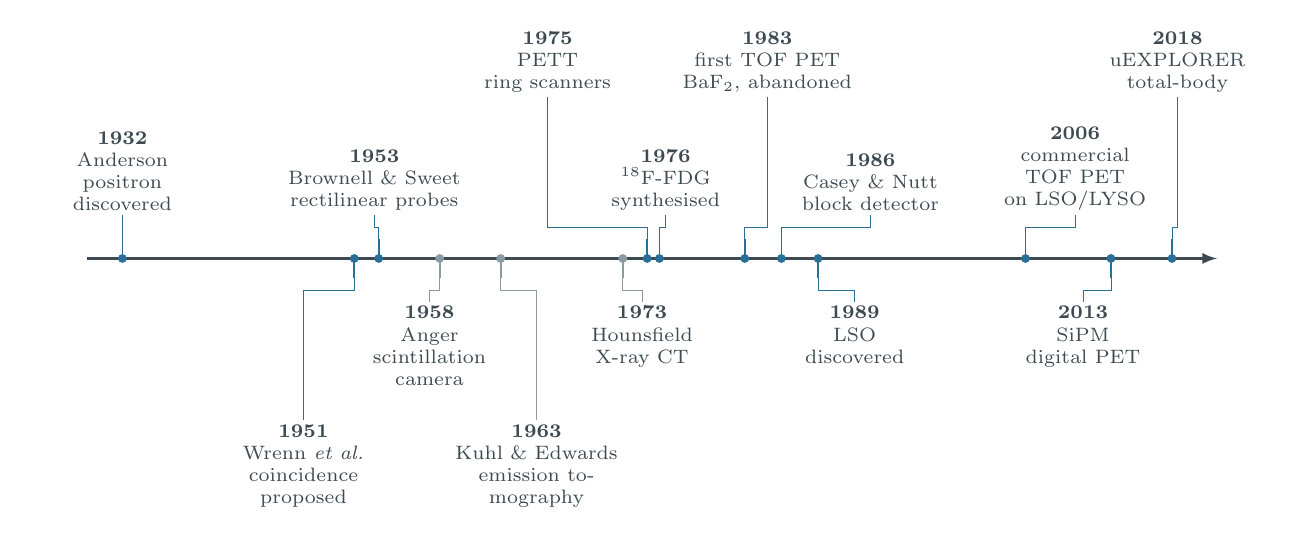
\begin{tikzpicture}[x=1cm, y=1cm, font=\scriptsize,
    tick/.style={line width=0.6pt},
    lead/.style={line width=0.3pt},
    lbl/.style={align=center, text width=2.3cm, text=tltext, inner sep=1.5pt,
                fill=white}]

\draw[tltext, line width=0.8pt, -latex] (-0.45,0) -- (13.9,0);

% --- positron line (above) --  year/row/label x/label ----------------------
\foreach \year/\r/\lx/\text in {%
    1932/1/0/{Anderson\\positron discovered},
    1953/1/3.2/{Brownell \& Sweet\\rectilinear probes},
    1975/2/5.4/{PETT\\ring scanners},
    1976/1/6.9/{\textsuperscript{18}F-FDG\\synthesised},
    1983/2/8.19/{first TOF PET\\BaF$_2$, abandoned},
    1986/1/9.5/{Casey \& Nutt\\block detector},
    2006/1/12.1/{commercial TOF PET\\on LSO/LYSO},
    2018/2/13.4/{uEXPLORER\\total-body}}
{
  \pgfmathsetmacro{\tx}{(\year-1932)*0.155}
  \pgfmathsetmacro{\lead}{0.55 + 1.50*(\r-1)}
  \draw[tlpositron, tick] (\tx,0) -- (\tx,0.25);
  \fill[tlpositron] (\tx,0) circle (1.6pt);
  \draw[tlpositron, lead] (\tx,0.25) -- (\tx,0.40) -- (\lx,0.40) -- (\lx,\lead);
  \begin{pgfonlayer}{tllabels}
    \node[lbl, anchor=south, name=n\year] at (\lx,\lead) {\textbf{\year}\\\text};
  \end{pgfonlayer}
}

% --- below the axis --  year/row/label x/colour/label ----------------------
% Mostly the borrowed single-photon and transmission lineage (tlsingle). The
% three tlpositron entries, 1951, 1989 and 2013, belong to the positron line
% but sit below purely for room: the upper track was carrying eleven of the
% fourteen milestones and needed a third row for them. They keep
% the positron colour so the two-track read survives the move -- track
% membership is carried by colour here, not by which side of the axis a label
% happens to sit on. Say so in the caption.
\foreach \year/\r/\lx/\col/\text in {%
    1951/2/2.3/tlpositron/{Wrenn \emph{et al.}\\coincidence proposed},
    1958/1/3.9/tlsingle/{Anger\\scintillation camera},
    1963/2/5.26/tlsingle/{Kuhl \& Edwards\\emission tomography},
    1973/1/6.6/tlsingle/{Hounsfield\\X-ray CT},
    1989/1/9.3/tlpositron/{LSO\\discovered},
    2013/1/12.2/tlpositron/{SiPM\\digital PET}}
{
  \pgfmathsetmacro{\tx}{(\year-1932)*0.155}
  \pgfmathsetmacro{\lead}{0.55 + 1.50*(\r-1)}
  \draw[\col, tick] (\tx,0) -- (\tx,-0.25);
  \fill[\col] (\tx,0) circle (1.6pt);
  \draw[\col, lead] (\tx,-0.25) -- (\tx,-0.40) -- (\lx,-0.40) -- (\lx,-\lead);
  \begin{pgfonlayer}{tllabels}
    \node[lbl, anchor=north, name=n\year] at (\lx,-\lead) {\textbf{\year}\\\text};
  \end{pgfonlayer}
}

% MEASUREMENT HOOK -- uncomment, then build with `tectonic --print` and grep
% the output for TLBOX to get every label's true bounding box in pt as
% (x0 y0 x1 y1). Two labels overlap iff their x ranges AND their y ranges
% both intersect; check every pair sharing a track. This is the only reliable
% way to catch collisions, since a label's real height depends on how many
% lines it wrapped to, which no arithmetic on the label x values predicts.
%
% \foreach \year in {1932,1951,1953,1958,1963,1973,1975,1976,1983,1986,1989,2006,2013,2018}{
%   \path (n\year.south west); \pgfgetlastxy{\xa}{\ya}
%   \path (n\year.north east); \pgfgetlastxy{\xb}{\yb}
%   \typeout{TLBOX \year\space \xa\space \ya\space \xb\space \yb}
% }
\end{tikzpicture}
